% This must be in the first 5 lines to tell arXiv to use pdfLaTeX, which is strongly recommended.
\pdfoutput=1
% In particular, the hyperref package requires pdfLaTeX in order to break URLs across lines.

\documentclass[11pt]{article}

% Remove the "review" option to generate the final version.
\usepackage{acl}
\usepackage{graphicx}
\graphicspath{ {./narrative_eye_tracking_analysis/images/} }
% Standard package includes
\usepackage{times}
\usepackage{latexsym}

% For proper rendering and hyphenation of words containing Latin characters (including in bib files)
\usepackage[T1]{fontenc}
% For Vietnamese characters
% \usepackage[T5]{fontenc}
% See https://www.latex-project.org/help/documentation/encguide.pdf for other character sets

% This assumes your files are encoded as UTF8
\usepackage[utf8]{inputenc}

% This is not strictly necessary, and may be commented out,
% but it will improve the layout of the manuscript,
% and will typically save some space.
\usepackage{microtype}

% If the title and author information does not fit in the area allocated, uncomment the following
%
%\setlength\titlebox{<dim>}
%
% and set <dim> to something 5cm or larger.

\title{An Analysis of Reader Engagement in Literary Fiction through Eye Tracking}


\author{Rose Neis \\
  University of Minnesota  \\
  \texttt{neis@umn.edu}
  \And
  Karin de Langis \\
  University of Minnesota\\
  \texttt{dento019@umn.edu} \\
  \AND
  Zae Myung Kim \\
  University of Minnesota\\
  \texttt{kim01756@umn.edu}
  \And
  Dongyeop Kang \\
  University of Minnesota\\
  \texttt{dongyeop@umn.edu} \\
  }

\begin{document}
\pagenumbering{arabic}
\maketitle

\begin{abstract}
Capturing readers' engagement in fiction is a challenging but important aspect of narrative understanding. In this study, we collected 23 readers’ reactions to 2 short stories through eye tracking, sentence-level annotations, and an overall engagement scale survey. Our aim is to analyze the significance of various qualities of the text in predicting how engaging a reader is likely to find it. As enjoyment of fiction is highly contextual, we will also investigate individual differences in our data. Furthering our understanding of what captivates readers in fiction will help better inform models used in creative narrative generation and collaborative writing tools.
\end{abstract}
\section{Introduction}
The question of reader engagement in fiction has been studied in the psychology field for decades, with some of the foundational theoretical work from Gerrig on Transportation Theory \citep{gerrig_1993} paving the way for more recent theoretical frameworks and experimental setups, which started in the early 2000s with the work by Green et al. interested in the role of transportation on the persuasiveness of narratives \citep{Green2004,green_brock_kaufman_2006}. In the past ten years, this question has been picked up in more fields, such as cognitive science, psycholinguistics, and computational narrative understanding, so we have more theoretical and experimental work to draw from.

However, as Arthur Jacobs emphasized in his article, "Towards a neurocognitive poetics model of literary reading", the samples normally collected are small and not enough to compensate for individual differences in reading patterns due to reader context and other situational factors \citep{willems_2015}. In order to help close the experimental gap, one contribution of this study is to provide the computational community with a data set of reader reactions to natural stories, which Jacobs refers to as "hot" experimental research.

In a 2009 study, a pair of researchers narrowed down the salient aspects of reader engagement, building off of Green's transportation framework to create narrative engagement scale \citep{busselle2009}, which we have modified slightly to gage overall interest in the story. In addition, in order to obtain more granular information, we used these aspects to design an annotation task that would provide sentence-level feedback. We use linear mixed models to discover textual features that have an impact on engagement and dwell time across readers.

\section{Related Research}
There have been several eye tracking and fMRI studies in the area of reader interest (a few are shown in \autoref{tab:first}). One small 5-participant study indicated some relationship between reading engagement and saccade angles as well as blink frequency \citep{kunze2015}. Another 13-participant study showed that words in enactive passages had on average longer fixation durations and dwell times \citep{Magyari2020}. Based on survey responses, the authors hypothesize that in the enactive texts, the ease of imagery contributes to greater involvement in imagination and results in an overall slower reading speed.

Then a much larger study in 2019 found a strong relationship between gaze durations and mental event descriptions correlated with subject’s scores on the Attention subscale of the Story World Absorption Scale (SWAS), as well as reported evoked responses and positive affect, indicating that absorption in the story correlates with longer gaze durations. An fMRI study found valence and arousal scores as good predictors of overall emotional experience of the reader. 


\begin{table*}[t]
\centering
\begin{tabular}{|c|c|c|c|c|c|c|}
\hline
& \textbf{Ours} & \textbf{Kunz et al.} & \textbf{Mangen et al.} & \textbf{Hsu et al.} & \textbf{Mak et al.} & \textbf{Maslej et al.} \\
\hline
\multicolumn{7}{|l|}{\textbf{Data gathered}}\\\hline
Eye tracking & x & x & x &  & x &  \\\hline
Saccade angle &  & x & x &  &  & \\\hline
fMRI &  &  &  & x &  & \\\hline
Engagement survey & x & x & x &  & x & x\\\hline
Engagement annotation & x &  &  & x &  & \\\hline
\multicolumn{7}{|l|}{\textbf{Textual features extracted}}\\\hline
Emotional arc & x &  &  &  &  & \\\hline
Lexical categories & x &  &  & x &  & x\\\hline
Description category &  &  & x &  &  & \\\hline

\end{tabular}
\caption{Comparison between our study and other similar experiments.}
\label{tab:first}
\end{table*}

\section{Research questions}

\subsection{RQ1: Does absorption in a story lead to longer gaze durations?}

Subquestion: do “Present” highlights (i.e. transported) correlate with faster reading and “Connected” and “Curious” highlights with slower reading as the Jacobs model hypothesized?

\subsection{RQ2: (move to future work) Does gaze duration increase in foregrounding passages and decrease in backgrounding passages?}

Subquestion: is absorption greater in foregrounding passages?

\subsection{RQ3: How much is engagement dependent on reader context vs. linguistic (discourse) features?}

What are the overlapping cases (sentences) when those two sets of features agree? What are the diverging cases? Can discourse features be used as a proxy for predicting eye-tracking features?

\subsection{RQ4: Are eye-tracking patterns consistent across users?}

If they are consistent, can we build a model using all of the users’ data to predict the engagement label or their future time-series data? If not, can we build separate models for each user? Analyses on diverging cases between the users: why are they diverging? Perhaps based on background, personal experience, interests, etc.

\subsection{RQ5: Is there a correlation between a sentence having low average word valence and reader’s absorption?}

\section{Methods}

\subsection{Participant study}

The study asked 31 English speakers (17 female, 11 male, 3 other, 23 native English speakers, average age: 26) were asked to read two short stories by Anton Chekhov while their eyes were tracked, and then answer an engagement scale survey. After reading through both stories, they completed a highlighting exercise where they highlighted areas according to the following categories:

\begin{itemize}
  \item Present: Able to vividly picture the scene in the story
  \item Confused
  \item Curious: Curious about what will happen next
  \item Connected: Connected to the character; able to identify with them or feel their emotions
  \item Other: Enjoyed it for a different reason
\end{itemize}

Due to calibration issues, 8 samples were discarded, leaving 23 (13 female, 8 male, 2 other, 17 native English speakers, average age: 28).

The eye tracking results were drift corrected and interest area reports were exported using words as interest areas. Outliers for dwell time were removed using inner quartile range (1.7\% of the data). The data was aggregated to the sentence level and dwell time values were normalized by sentence character count. To handle missing data, null values for the eye tracking features were filled with the average of the 5 nearest sentences (5.7\% of all sentences read across participants).

\begin{figure*}
  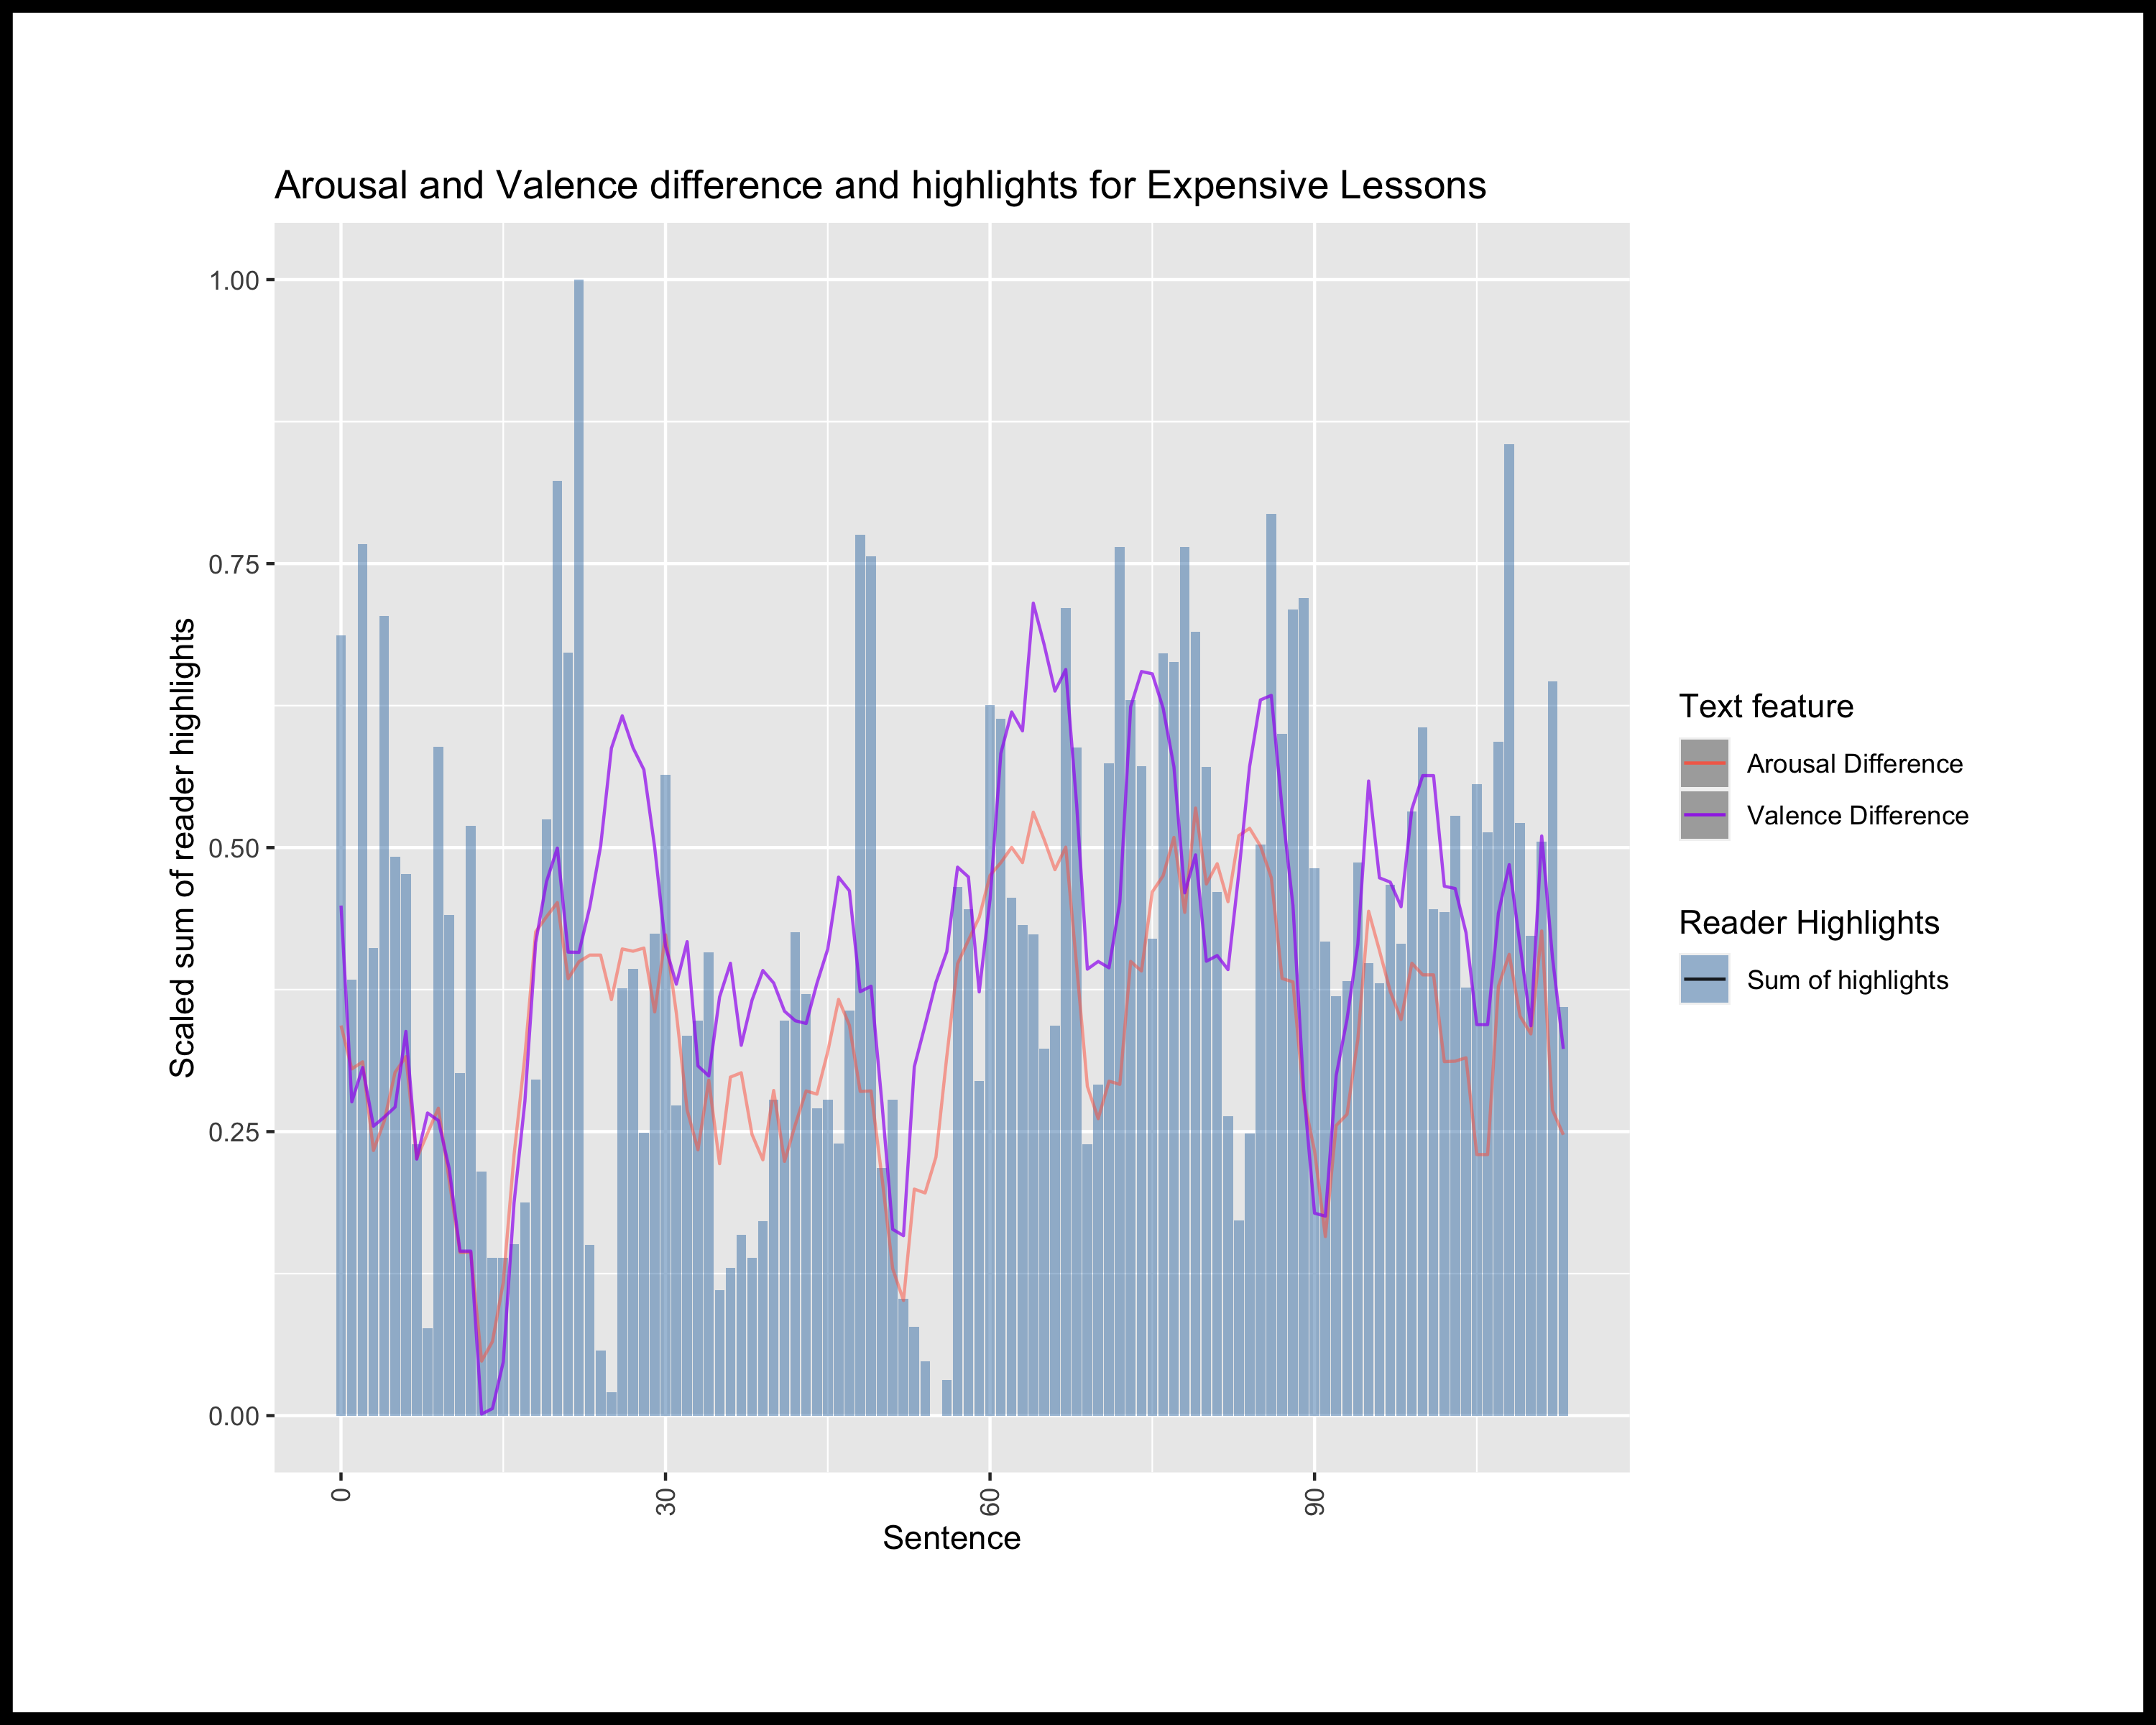
\includegraphics[height=6cm]{el_highlights_val_arousal}
  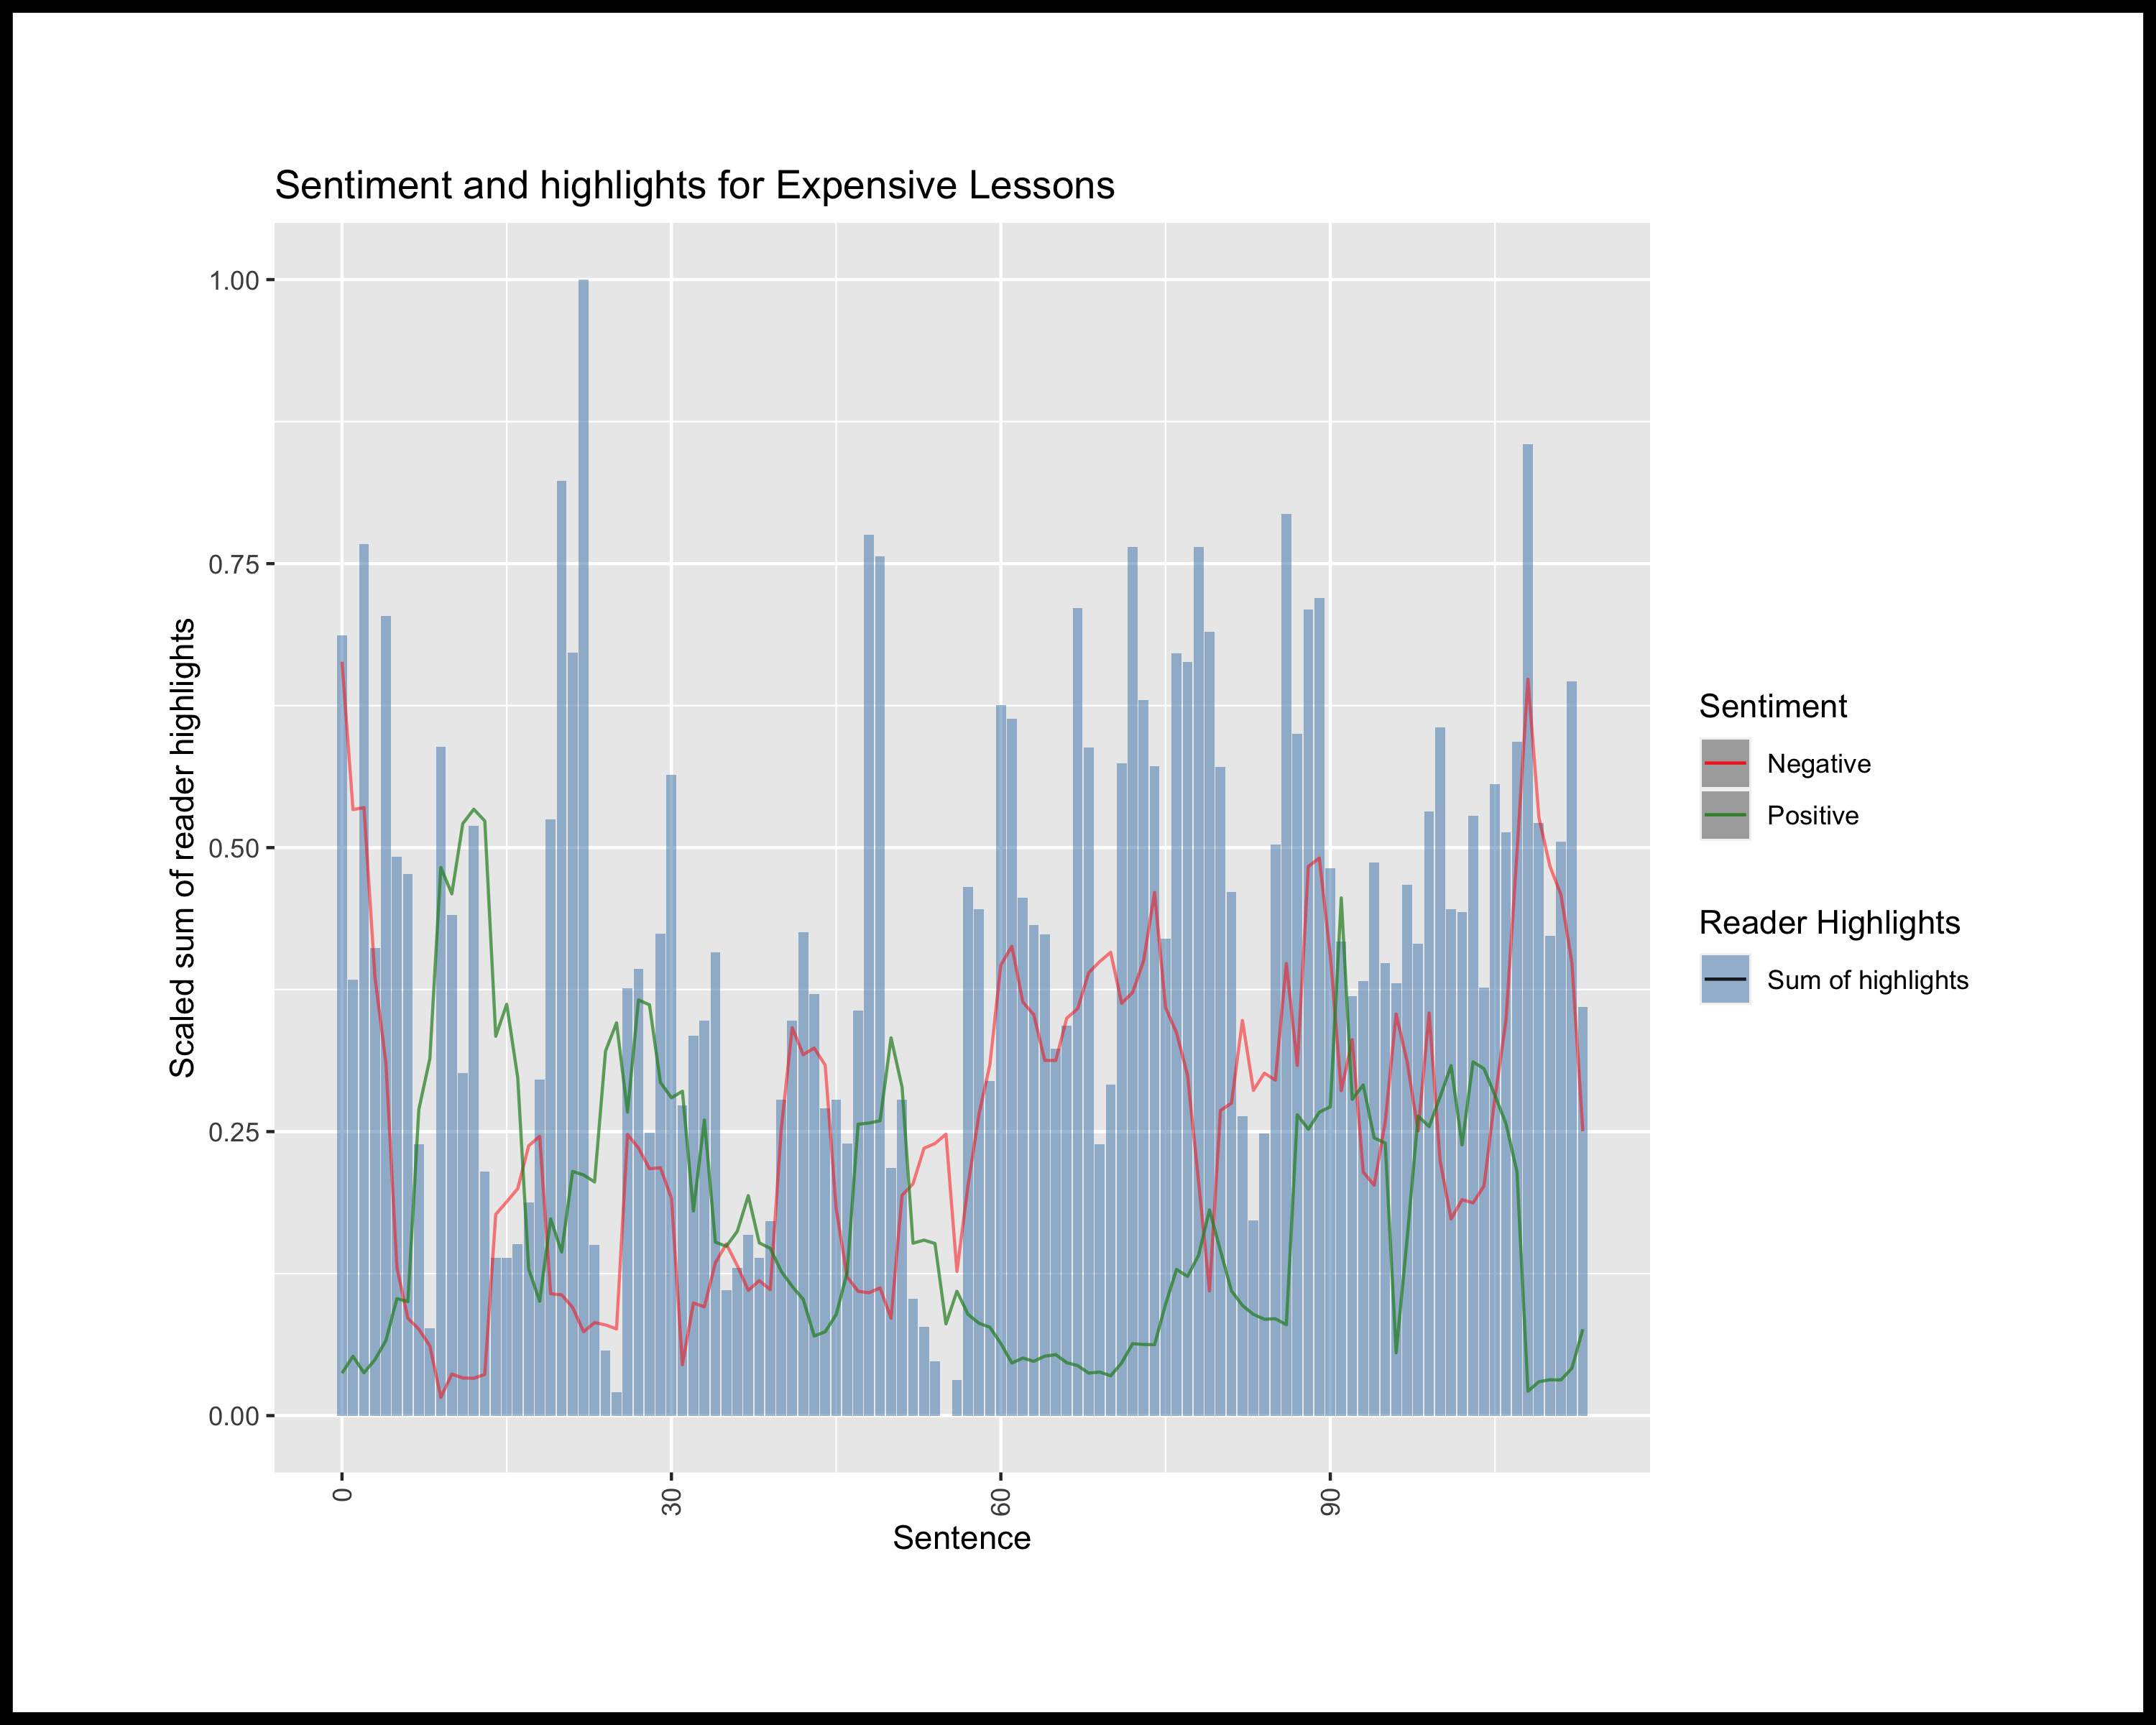
\includegraphics[height=6cm]{el_highlights_sentiment}
  \caption{Highlights and features.}
\end{figure*}

\subsection{Linguistic and discourse features}

We extracted the following features from the stories to create sentence-level predictors: sentiment scores using the RoBERTa sentiment base model (footnote with link to huggingface), emotion categories using the DistilRoBERTa emotion base model, concreteness from the Brysbaert (brysbaert2014) corpus, valence and arousal from the NRC-VAD corpus, word frequency from the subtlex corpus, and average word length.

\section{Limitations}

There is an imbalance in how many participants read each story first (Expensive Lessons: 16, Schoolmistress: 7), which may affect level of attention for the second story. In addition, the stories did not receive very high scores on average in the engagement survey. On a scale from 0-4, Expensive Lessons got an average of 2.09 and Schoolmistress got 1.92.

\section{Results}

Other studies have shown that valence and arousal play an important role in predicting interest in a story (Maslej, Jacobs 2015, HSU201596) and Jacobs emphasized the importance of affective and emotional processes. We used linear mixed models to fit predictions of the proportion of the sentence highlighted and gaze duration, with random effects of participant (n=23) and story (n=2). For predicting the proportion of a sentence highlighted, a proxy for a higher level of engagement, our results support a slight significance of valence mean (p=0.0049), similar to Hsu.

\begin{table*}[t]
  \centering
  \begin{tabular}{|l|r|r|r|r|r|r|}
  \hline
   & Estimate & Std. Error & df & t value & $Pr(>|t|)$ & Sig. \\
  \hline
  (Intercept) & 0.01910 & 0.07439 & 220.85084 & 0.257 & 0.797621 & \\
  character count & 0.15837 & 0.03851 & 7070.78993 & 4.112 & $3.97 \times 10^{-5}$ & $\ast\ast\ast$ \\
  word frequency avg. & 0.06215 & 0.09899 & 7094.55339 & 0.628 & 0.530152 & \\
  positive & 0.03362 & 0.02244 & 7120.97997 & 1.498 & 0.134154 & \\
  negative & 0.10018 & 0.02035 & 7112.05570 & 4.923 & 8.74e-07 & $\ast\ast\ast$ \\
  concreteness & 0.01150 & 0.01361 & 6942.09621 & 0.845 & 0.398257 & \\
  valence avg. & 0.12612 & 0.04488 & 7120.08454 & 2.810 & 0.004964 & $\ast\ast$ \\
  arousal avg. & -0.03312 & 0.05385 & 7118.47514 & -0.615 & 0.538580 & \\
  valence diff. & 0.10635 & 0.02634 & 7118.61978 & 4.037 & $5.47 \times 10^{-5}$ & $\ast\ast\ast$ \\
  arousal diff. & 0.11636 & 0.03165 & 7064.83819 & 3.677 & 0.000238 & $\ast\ast\ast$ \\
  \hline
\end{tabular}
\caption{Fixed Effects for predicting proportion of sentence highlighted}
\label{tab:second}
\end{table*}

Unlike in other studies, we found that arousal mean had no significance (p=0.598).  However, like Hsu, there was a higher significance for valence-span (p=0.00003) - the difference between valence max and valence min and arousal-span (p=0.00029) - the difference between arousal max and arousal min. This suggests that the reader was more engaged in sentences with a higher range of valence and arousal. Other features that had an effect were negative sentiment score (p=8.74e-07) and character count (p=3.97e-05). This model explains 22.9\% of the variance in the proportion of a sentence highlighted with random effects and 3.6\% without.

\begin{table*}[t]
  \centering
  \begin{tabular}{|l|r|r|r|r|r|r|}
  \hline
  & Estimate & Std. Error & df & t value & $Pr(>|t|)$ & Sig. \\
  \hline
  (Intercept) & 0.1255 & 0.0233 & 91.28 & 5.396 & 5.34e-07 & $\ast\ast\ast$ \\
  word frequency avg. & 0.5548 & 0.0297 & 7117 & 18.656 & $< 2 \times 10^{-16}$ & $\ast\ast\ast$ \\
  positive & 0.0251 & 0.0068 & 7117 & 3.707 & 0.000211 & $\ast\ast$ \\
  negative & 0.0191 & 0.0061 & 7116 & 3.121 & 0.001813 & $\ast\ast$ \\
  concreteness & 0.0146 & 0.0041 & 7086 & 3.568 & 0.000362 & $\ast\ast$ \\
  valence avg. & -0.0896 & 0.0135 & 7117 & -6.655 & $3.03 \times 10^{-11}$ & $\ast\ast\ast$ \\
  arousal avg. & 0.0147 & 0.0161 & 7117 & 0.914 & 0.360620 & \\
  valence diff. & -0.0396 & 0.0075 & 7116 & -5.306 & $1.16 \times 10^{-7}$ & $\ast\ast\ast$ \\
  arousal diff. & -0.0801 & 0.0089 & 7117 & -9.026 & $< 2 \times 10^{-16}$ & $\ast\ast\ast$ \\
  proportion & -0.0021 & 0.0036 & 7141 & -0.598 & 0.550015 & \\
  \hline
  \end{tabular}
  \caption{Fixed Effects for predicting gaze duration}
  \label{tab:third}
  \end{table*}

In predicting gaze duration, valence mean had a slight significance (p=0.0181) and arousal mean had none (p=0.365) and valence-span (p=0.0336) had a slight significance while arousal-span was found to be significant, but with a negative slope (p=0.00047). These findings do not support Jacobs's proposed framework, which states that passages that engage our emotions would likely result in slower reading. However, we found a positive relationship with negative sentiment (p=0.0048), which may partially support his proposal that the affective mode of reading is more readily triggered by negative emotion. Length of the sentence (p=0.000012) and word frequency (p=0.000048) were the most significant predictors of dwell time. This model explains 30.15\% of the variance in the proportion of a sentence highlighted with random effects and 0.7\% without.



\section{Future Work}


Investigate: Does gaze duration increase in foregrounding passages and decrease in backgrounding passages?

\section{Conclusion}


\subsection{References}

\nocite{Green2004,liwc_22,kuzmicova2014,brysbaert2014,Maslej2019TheTF,green_brock_kaufman_2006,Consoli2018,busselle2009,jacobs2018,jacobs2017,stockwell2002cognitive,HSU201596,willems_2015,mak2019,kunze2015,ferreira-goncalo-oliveira-2018-seeking,aryani2013,delatorre2019,andrade2020,indico2015,gerrig_1993,Magyari2020}

\bibliographystyle{acl_natbib}
\bibliography{anthology,custom}


\section*{Acknowledgements}

We would like to thank the Text Group for initial feedback on experiment setup and the Blue Lantern Writing Group for additional feedback.

\end{document}